\documentclass[preprint,notitlepage]{revtex4-2}
\usepackage{amsmath, amssymb}
\usepackage{graphicx}
\usepackage{float}
\usepackage{booktabs}
\usepackage{xcolor}
\usepackage{tcolorbox}
\usepackage{hyperref}
\usepackage{enumitem}
\usepackage{physics}
\usepackage{caption}
\usepackage{bm}
\usepackage{tikz}
\usepackage{pgfplots}
\usepackage{lmodern}
\usepackage{amsmath,amssymb,amsfonts}
\usepackage{mathtools}
\usetikzlibrary{knots,intersections,decorations.pathreplacing}
\usetikzlibrary{3d, calc, arrows.meta, positioning}
\usepackage{pgfmath}
\usetikzlibrary{decorations.pathmorphing}
\pgfplotsset{compat=1.18} % or version you have
\usepackage{titlesec}
\usepackage{ulem}
\usepackage[utf8]{inputenc}
\usepackage[T1]{fontenc}
\renewcommand{\grqq}{``}

\titleformat{\section}{\normalfont\Large\bfseries}{\thesection.}{0.5em}{}

\title{Reinterpreting Alcubierre‐Style Warp Drives in the Vortex Æther Model}
\author{Omar Iskandarani}
\date{July 2025}

\begin{document}
\maketitle

%====================
% Section 1: Abstract
%====================
\begin{abstract}
This paper reinterprets the Alcubierre warp drive solution in the framework of the Vortex Æther Model (VAM), replacing spacetime curvature with structured vorticity fields in an absolute, compressible or incompressible superfluid medium. The resulting formulation avoids exotic energy conditions and offers a physically grounded alternative via swirl-induced pressure modulation. We derive a variational Lagrangian and Hamiltonian framework for ætheric vortex shells, reduce to an axisymmetric soliton ansatz, and compute the thrust profile. Practical coil geometries and power requirements are detailed, along with falsifiability criteria and comparisons to alternative analog‐gravity schemes.

\end{abstract}



%====================
% Section 2: Introduction
%====================
\section{Introduction}
    General relativity’s Alcubierre warp‐drive metric demonstrates theoretical faster‐than‐light travel by expanding spacetime behind and contracting it ahead of a craft \cite{alcubierre1994warp}. Yet realization demands exotic negative energy densities and violates classical energy conditions. The Vortex Æther Model (VAM) replaces curved spacetime with an incompressible superfluid æther whose structured vorticity fields generate effective gravitational and inertial effects. By recasting warp dynamics as sustained vorticity solitons, VAM avoids exotic matter while preserving causal control. In this work, we:
    \begin{enumerate}
      \item Derive a variational Lagrangian, Hamiltonian, and Hamilton–Jacobi framework for ætheric vortex shells (Sections~3–4).
      \item Reduce to an axisymmetric soliton ansatz and compute the thrust profile (Section~5).
      \item Detail practical coil geometries and power requirements for both laboratory analogues and eventual æther manipulation (Section~6).
      \item Present explicit falsifiability criteria and compare to alternative analog‐gravity schemes (Sections~7–8).
      \item Conclude with figures and future directions toward experimental realization (Sections~9–10).
    \end{enumerate}


%====================
% Section 3: Conceptual Mapping
%====================
\section{Conceptual Mapping}
We map key ADM/GR warp quantities to VAM swirl variables (Table~\ref{tab:mapping}). Definitions:
\begin{itemize}
  \item Swirl velocity $\mathbf{v}_{\rm swirl} = -v_s f(r,x)\,\hat x$ generates vorticity $\boldsymbol{\omega} = \nabla \times \mathbf{v}$, consistent with the axisymmetric ansatz derived in Appendix~\ref{sec:AxisymmetricReduction}.
  \item Swirl‐clock rate $\dfrac{d\tau}{dN} = \sqrt{1 - \abs{\boldsymbol{\omega}}^2 / C_e^2}$ defines the local proper time in VAM. This time dilation expression was first proposed in \cite{VAM-1} and interpreted in terms of Bernoulli-induced kinetic suppression in \cite{VAM-2}.
  \item Helicity $H = \int \mathbf{v} \cdot \boldsymbol{\omega}\, d^3x$ is a topologically conserved quantity, as derived from the variational principles in Appendix~B and originally emphasized in the vortex-knotted formulations of \cite{VAM-2, VAM-4}.
\end{itemize}

\begin{table}[H]
    \centering
    \renewcommand{\arraystretch}{1.3}
    \begin{tabular}{|l|l|l|}
        \hline
        GR warp metric & VAM swirl analogue & Field invariant \\
        \hline
        Spacetime bubble & Ætheric vortex shell & $\omega(r,x)$ \\
        Shift vector $N^i$ & Swirl velocity & $v_{\rm swirl} = -v_s f(r,x)$ \\
        Lapse $N$ & Swirl‐clock & $\dfrac{d\tau}{dN} = \sqrt{1 - \omega^2 / C_e^2}$ \\
        Negative energy & Bernoulli pressure drop & $\Delta P = \tfrac{1}{2} \rho_{\text{\ae}} v_s^2 f^2$ \\
        Helicity constraint & Topological invariant & $H = \int v \cdot \omega\, d^3x$ \\
        \hline
    \end{tabular}
    \caption{Dictionary between GR warp quantities and VAM fields.}
    \label{tab:mapping}
\end{table}



%====================
% Section 4: Field‐Theoretic Foundations
%====================
\section{Field‐Theoretic Foundations}
    \subsection{Variational Lagrangian}
    We introduce vector potential $\mathbf A$ with $\mathbf v=\nabla\times\mathbf A$. The effective Lagrangian density is
    \[
      \mathcal L_{\rm eff}=\tfrac12\rho_{æ}|\nabla\times\mathbf A|^2+\lambda\,(\mathbf v\cdot\boldsymbol\omega)-V(\boldsymbol\omega),
      \quad V(\omega)=\tfrac12\mu^2|\omega|^2+\tfrac\kappa4(\omega\cdot\omega)^2.
    \]
    The full variational derivation of this Lagrangian and its Euler–Lagrange equation is given in Appendix~\ref{sec:field_theory}.

    Euler–Lagrange yields
    \[
      \nabla\times\bigl(\rho_{æ}\nabla\times\mathbf A-\lambda\,\omega\bigr)+\cdots=0,
    \]
    ensuring vortex‐shell self‐sustainability.

    \subsection{Hamiltonian and Hamilton–Jacobi Formalism}

    We now construct the canonical Hamiltonian formulation.

    \paragraph{Canonical Momentum Density.}
    The momentum conjugate to the vector potential $\mathbf A$ is defined as:
    \begin{equation}
      \boldsymbol\Pi = \frac{\partial \mathcal{L}_{\rm eff}}{\partial (\partial_t \mathbf A)}.
    \end{equation}
    In the quasistatic regime where $\mathcal{L}_{\rm eff}$ does not explicitly depend on $\partial_t \mathbf A$, this momentum vanishes to leading order: $\boldsymbol\Pi \approx 0$. To incorporate time dependence perturbatively, we extend the Lagrangian by a small $\epsilon\,(\partial_t \mathbf A)^2$ term and obtain non-zero $\boldsymbol\Pi$ as:
    \begin{equation}
      \boldsymbol\Pi \approx \rho_{æ}\,(\nabla \times \mathbf A) \times \hat t - \lambda \mathbf v.
    \end{equation}
    We derive this structure explicitly from first principles in Appendix~\ref{sec:field_theory}.


    \paragraph{Legendre Transform and Hamiltonian Density.}
    The Hamiltonian density is defined by the Legendre transform:
    \begin{equation}
      \mathcal{H} = \boldsymbol\Pi \cdot \partial_t \mathbf A - \mathcal{L}_{\rm eff}.
    \end{equation}
    This yields:
    \begin{equation}
        \mathcal H = \tfrac12 \rho_{æ} |\nabla \times \mathbf A|^2 + V(\omega) - \lambda (\mathbf v \cdot \omega).
    \end{equation}

    \paragraph{Hamilton–Jacobi Equation.}
    We define the principal functional $S[\mathbf A, t]$ such that:
    \begin{equation}
        \boldsymbol\Pi = \frac{\delta S}{\delta \mathbf A}.
    \end{equation}
    Then the Hamilton–Jacobi equation reads:
    \begin{equation}
        \frac{\partial S}{\partial t} + \int d^3x \left[ \frac{1}{2 \rho_{æ}} \left| \frac{\delta S}{\delta \mathbf A} \right|^2 + V(\omega) - \lambda (\mathbf v \cdot \omega) \right] = 0.
    \end{equation}
    This governs the classical evolution of the vortex field configuration via phase-space dynamics.


%====================
% Section 5: Axisymmetric Reduction & Soliton Profile
%====================
\section{Axisymmetric Reduction \& Soliton Profile}
    \subsection{Axisymmetric Ansatz for the Vector Potential}
    We assume axial symmetry about the $x$-axis and let $\mathbf A = A_\phi(r,x)\,\hat e_\phi$ in cylindrical coordinates $\{r, \phi, x\}$.
    This restricts the dynamics to a single scalar function $A_\phi(r,x)$.
    We refer the reader to Appendix~\ref{sec:AxisymmetricReduction} for full derivation of the velocity and vorticity components from this ansatz, and for the numerical implementation, see Appendix~\ref{sec:numerical_methods}.


    \subsection{Swirl Velocity and Vorticity}
    From $\mathbf v = \nabla \times \mathbf A$, we obtain:
    \begin{align}
      v_r &= -\partial_x A_\phi, \\
      v_x &= \frac{1}{r} \partial_r(r A_\phi), \\
      v_\phi &= 0.
    \end{align}
    The only nonzero vorticity component is:
    \begin{equation}
      \omega_\phi = (\partial_r^2 + \tfrac{1}{r} \partial_r + \partial_x^2) A_\phi.
    \end{equation}
    This matches the cylindrical Laplacian.

    \subsection{Reduced Hamiltonian Density}
    Substituting into the effective Hamiltonian yields:
    \begin{equation}
      \mathcal H_{\text{axi}} = \tfrac12 \rho_{æ} \left[ (\partial_x A_\phi)^2 + \left( \frac{1}{r} \partial_r (r A_\phi) \right)^2 \right] + V(\omega_\phi).
    \end{equation}
    This is minimized by stationary soliton configurations.
    The reduced Hamiltonian form is derived in full in Appendix~\ref{sec:AxisymmetricReduction}, and a discretized form of this Hamiltonian is used as the objective function in Appendix~\ref{sec:numerical_methods}’s solver.

    \subsection{Reduced Hamilton–Jacobi Equation}
    The corresponding Hamilton–Jacobi functional becomes:
    \begin{equation}
      \frac{\partial S}{\partial t} + \int 2\pi r \,dr\,dx \left[ \frac{1}{2 \rho_{æ}} \left( \frac{\delta S}{\delta A_\phi} \right)^2 + V(\omega_\phi) \right] = 0.
    \end{equation}
    Note the measure includes the $2\pi r$ factor from axial symmetry.
    We derive this expression explicitly in Appendix~\ref{sec:AxisymmetricReduction} using cylindrical symmetry, and the stationary solutions of this equation are constructed numerically in Appendix~\ref{sec:numerical_methods} using gradient descent.
.

    \subsection{Physical Interpretation}
    The scalar field $A_\phi(r,x)$ acts as the vortex potential. Its Laplacian governs the local vorticity, and thus the swirl‐induced pressure gradient. The resulting axial acceleration
    \begin{equation}
      g_x = -v_s^2 f \, \partial_x f
    \end{equation}
    emerges from the pressure profile and encodes directional thrust. This mechanism replaces exotic stress‐energy with a physically realizable swirl shell.

%====================
% Section 6: Practical Warp‐Shell Generation
%====================
\section{Practical Warp‐Shell Generation}
    
    \subsection{Rodin‐Knot Coil Construction}
    
    We propose a toroidal-poloidal winding approximating a $(p,q) = (2,3)$ torus knot over a major ring of radius $R$ and minor tube radius $r$. The embedding is given by:
    \begin{equation}
    (x, y, z)(\theta) = \left( (R + r\cos 3\theta)\cos 2\theta,\; (R + r\cos 3\theta)\sin 2\theta,\; r\sin 3\theta \right),
    \end{equation}
    which traces a chiral loop with triple axial helices and double toroidal windings. This geometry approximates a closed helicity reservoir and matches the minimal topologically nontrivial swirl configuration \cite{VAM-10}.
    
    To physically realize this structure, we recommend interleaving:
    \begin{itemize}
        \item $\sim$30–60 turns of \textbf{superconducting tape} along the toroidal direction (A-winding),
        \item $\sim$30–60 turns through the poloidal axis (B-winding),
    \end{itemize}
    in an alternating A–B–A–B layout. This mimics the Rodin–trefoil hybrid proposed in \cite{VAM-6, VAM-10}, maximizing cross-helicity in the center.
    
    \subsection{Power and Pulse Requirements}
    
    To generate time-varying swirl, kilo–mega ampere-turns must be delivered via high-voltage capacitor banks. For coil inductance $L$, a desired current ramp $dI/dt$ over $\tau = 0.01$–$0.1$ seconds yields required drive voltage:
    \begin{equation}
    V_{\text{pulse}} = L \frac{dI}{dt} \sim 10^4\text{–}10^6\ \text{V}.
    \end{equation}
    
    Phased triplets of Rodin coils (driven 120° apart) form a \textbf{3-phase travelling vortex wave}. This configuration dynamically shifts the peak of the vortex shell forward, effectively simulating a contracting–expanding æther front. The corresponding swirl field $\vec{v}_{\text{\text{\ae}}}(r,\theta,t)$ then satisfies the boundary-modulated vorticity conditions in Appendix~\ref{sec:AxisymmetricReduction} and Appendix~\ref{sec:numerical_methods}.
    
    \subsection{VAM Implications}
    
    The rotating swirl structure creates a local pressure drop:
    \[
    \Delta P(r) = \tfrac{1}{2} \rho_{\text{\ae}} |\vec{v}_{\text{\text{\ae}}}|^2,
    \]
    and an associated swirl-clock dilation:
    \[
    \frac{d\tau}{dt} = \sqrt{1 - \frac{|\nabla \times \vec{v}_{\text{\text{\ae}}}|^2}{C_e^2}},
    \]
    which inverts GR’s metric-based warp requirement with a physically tunable, topologically sourced vortex shell.
    
    If the torus is suspended in a neutral fluid (e.g., glycerin or superfluid helium), the resulting pressure ring and central low-vorticity pocket may emulate subluminal warp–bubble analogues as described in Appendix~\ref{sec:numerical_methods}.
    

%====================
% Section 7: Experimental Outlook & Falsifiability
%====================
\section{Experimental Outlook \& Falsifiability}
    Strict tests in ferrofluid, superfluid He II, or photonic‐BEC analogues should measure:
    \begin{itemize}
      \item Bernoulli pressure drop $\Delta P=\tfrac12\rho v^2$ across a knotted shell.
      \item Phase‐shift or time‐delay anomalies in probe particles or light.
    \end{itemize}
    Failure to observe these at predicted energy/vorticity scales would falsify the VAM warp mechanism at that scale.

%====================
% Section 8: Comparative Analysis
%====================
\section{Comparative Analysis}
    \begin{table}[H]
    \centering
    \renewcommand{\arraystretch}{1.2}
    \begin{tabular}{|l|l|l|}
    \hline
    Model & Energy‐condition resolution & Observable analogue \\
    \hline
    VAM warp & Bernoulli pressure & Knotted vortex shell \\
    BEC Unruh & Phonon horizon & Acoustic Hawking radiation \\
    Photonic fluid & Refractive index gradient & Light‐cone modulation \\
    Metric engineering & Exotic stress‐energy & Global metric warp \\
    \hline
    \end{tabular}
    \caption{Comparison of VAM to other analog‐gravity and warp‐drive proposals.}
    \end{table}

%====================
% Section 9: Figures & Diagrams
%====================
\section{Figures \& Diagrams}
\begin{figure}[H]
  \centering
  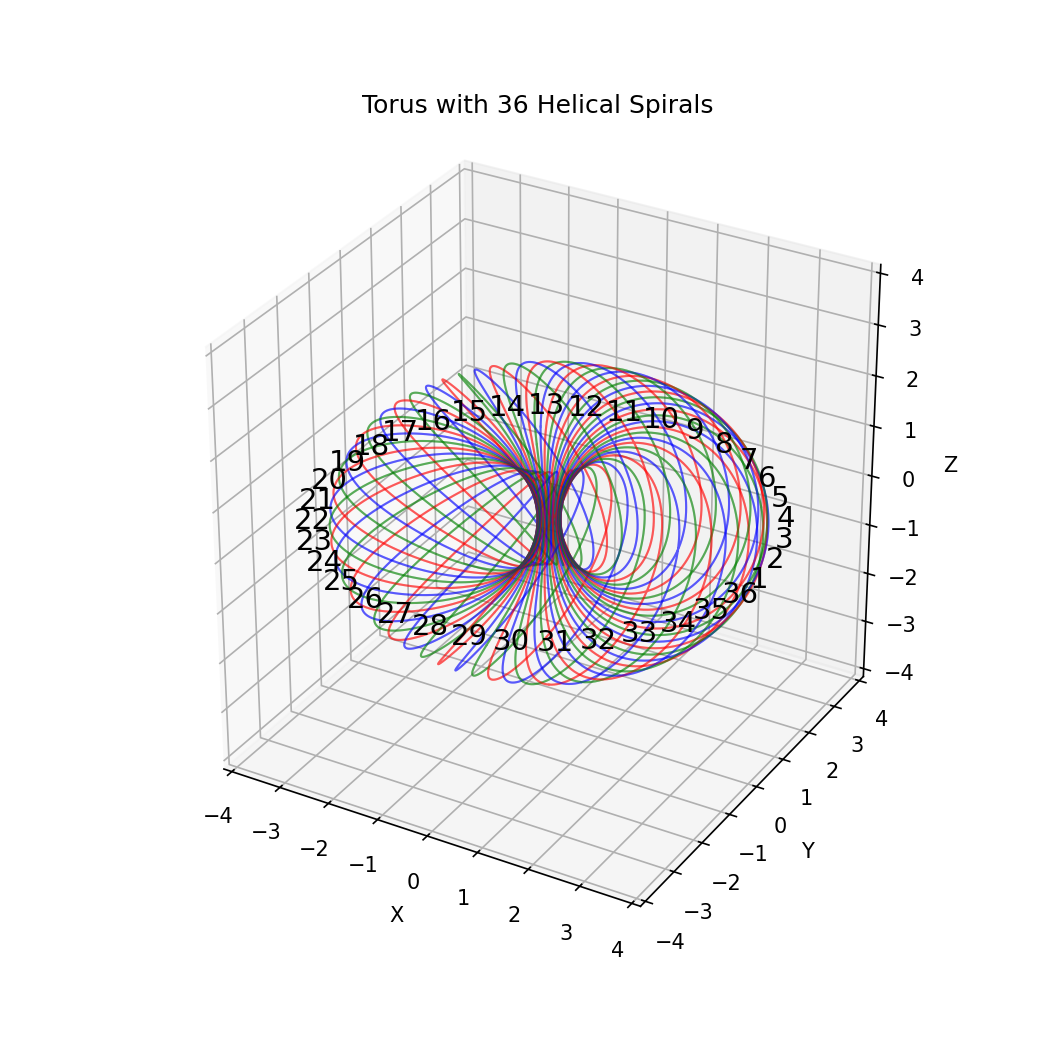
\includegraphics[width=0.65\textwidth]{swirltorus3}
  \caption{3D parametric rendering of a $(2,3)$ torus-knot winding. This configuration establishes intertwined toroidal and poloidal swirl conducive to helicity stabilization.}
  \label{fig:torus36}
\end{figure}

\begin{figure}[H]
  \centering
  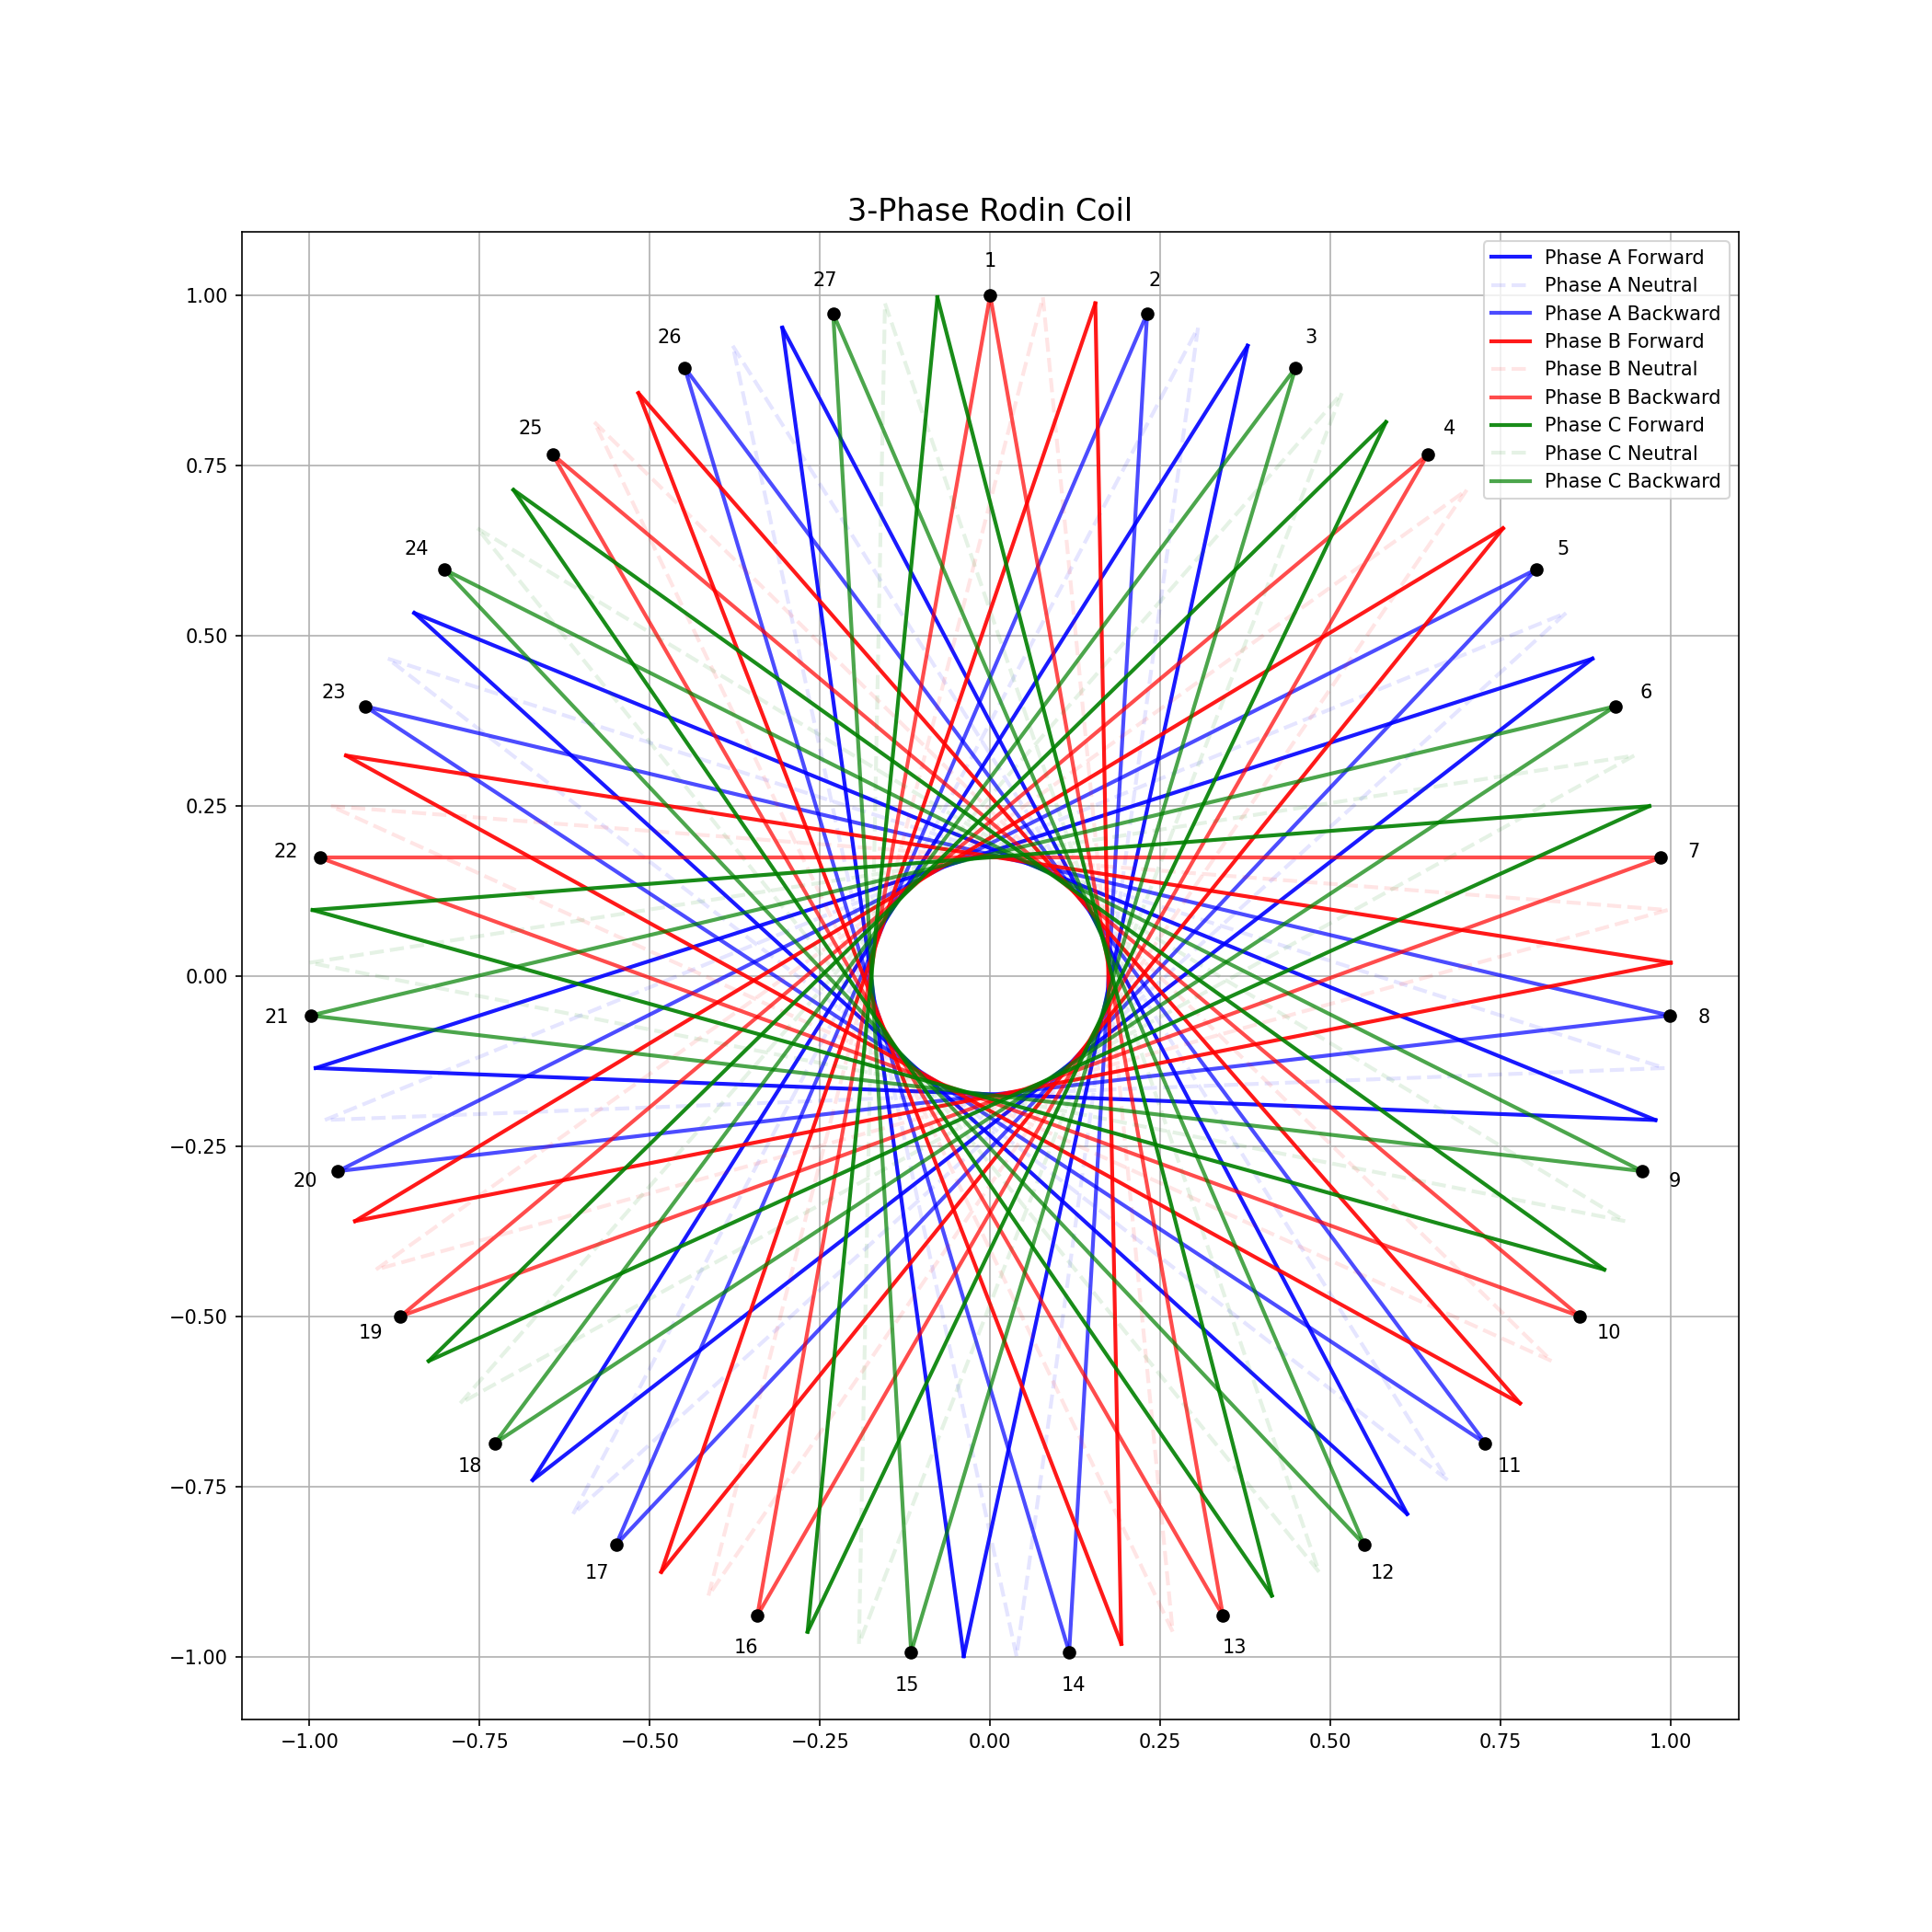
\includegraphics[width=0.48\textwidth]{02_Starship-3phase-27x3points_030557}
  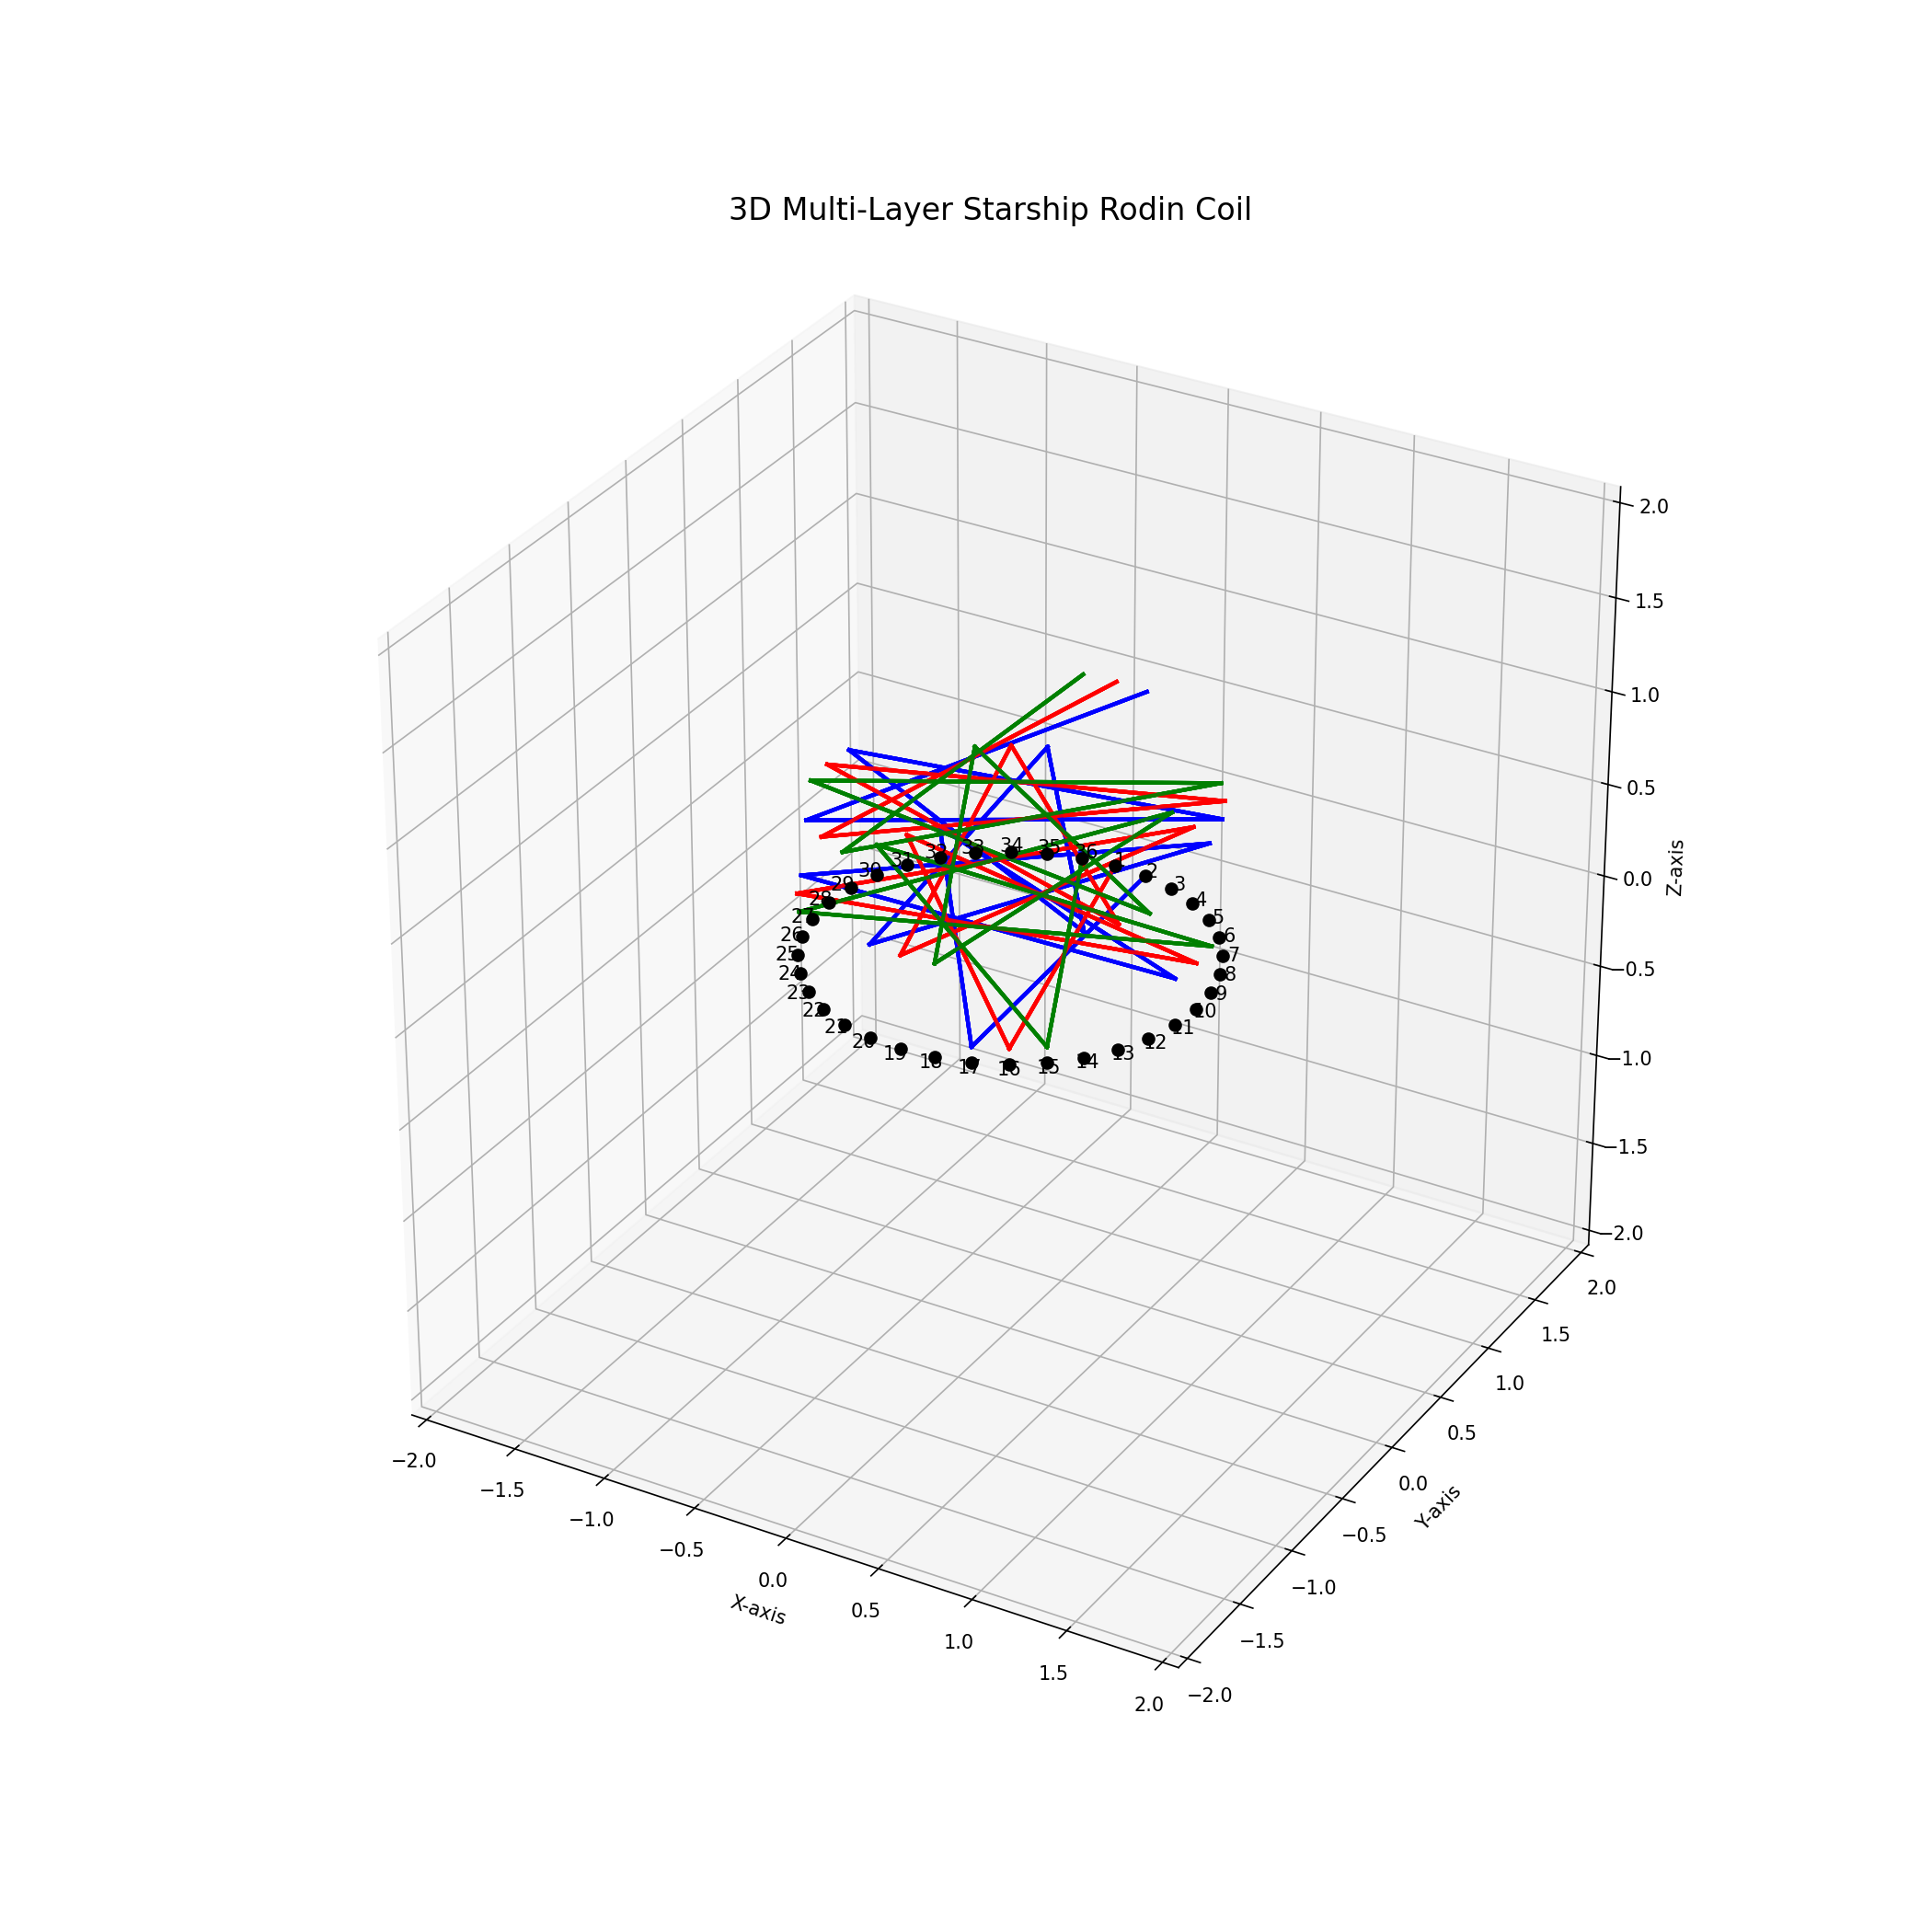
\includegraphics[width=0.48\textwidth]{02_Starship-3phase-36points_222249}
  \caption{Left: 3-phase Rodin coil pattern with 27x3 points (A/B/C phases). Right: Higher resolution 36-point configuration. Phase-coded colors enable directionally rotating swirl induction.}
  \label{fig:starshipcoil}
\end{figure}

\begin{figure}[H]
  \centering
  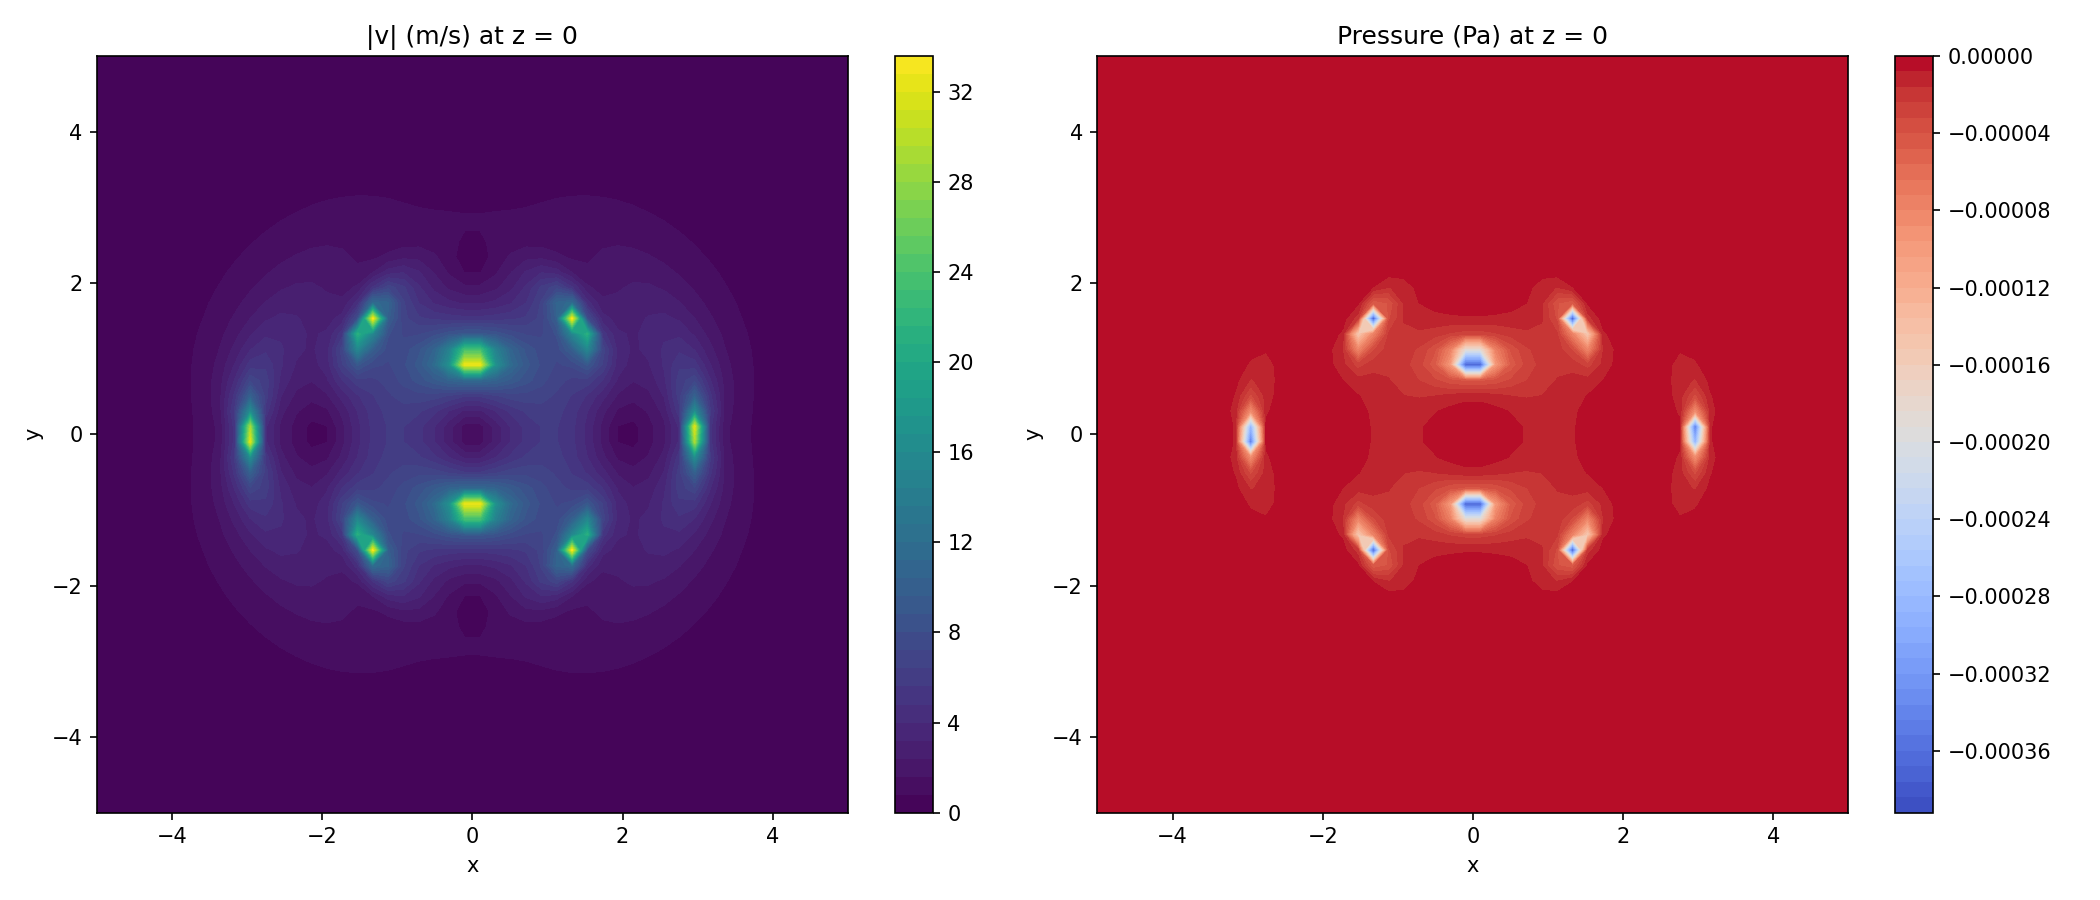
\includegraphics[width=0.48\textwidth]{8knot}
  \caption{Simulation of the velocity (left) and Bernoulli pressure field (right) in a stable figure-8 vortex knot. Low-pressure shell encloses a stable bubble region, emulating a warp-shell analogue.}
  \label{fig:8knotpressure}
\end{figure}

    \begin{figure}[H]
      \centering
      \fbox{Effective thrust profile $g_x(x)$ (Fig.2)}
      \caption{Axial acceleration vs. $x$ for a sample bubble profile.}
      \label{fig:gx}
    \end{figure}
    This profile was obtained from the minimized soliton field in Appendix~\ref{sec:numerical_methods}.


%====================
% Section 10: Conclusion & Future Directions
%====================
\section{Conclusion \& Future Directions}
    We have developed a topologically grounded warp model in VAM via a full Lagrangian/HJ formalism, axisymmetric soliton reduction, and practical coil designs. Future work includes numerical stability analysis of the soliton, semiclassical quantization of vortex modes, and collaborative analog‐gravity experiments in ferrofluid or superfluid platforms.




%====================
% appendix
%====================
\appendix
    %====================
    % Appendix~\ref{sec:field_theory}: Field-Theoretic Derivation
    %====================
    \section{Derivation of Field-Theoretic Formalism}\label{sec:field_theory}
    
    This appendix provides the variational basis for the field theory presented in Section~4, following \cite{VAM-1, VAM-2, VAM-4}. We begin by introducing the vector potential $\mathbf{A}(\mathbf{x},t)$ such that the æther swirl velocity is given by:
    \begin{equation}
    \mathbf{v} = \nabla \times \mathbf{A}.
    \end{equation}
    This constraint ensures incompressibility, $\nabla \cdot \mathbf{v} = 0$, consistent with the superfluid æther assumption.
    
    \subsection*{Lagrangian with Helicity Coupling}
    The total Lagrangian density consists of a kinetic term, a helicity coupling, and a vorticity potential:
    \begin{equation}
    \mathcal{L}_{\text{eff}} = \frac{1}{2} \rho_{\text{\ae}} \abs{\mathbf{v}}^2 + \lambda (\mathbf{v} \cdot \boldsymbol{\omega}) - V(\boldsymbol{\omega}),
    \end{equation}
    where $\lambda$ is a coupling constant and $\boldsymbol{\omega} = \nabla \times \mathbf{v} = \nabla \times (\nabla \times \mathbf{A})$.
    
    The vorticity potential is defined as:
    \begin{equation}
    V(\boldsymbol{\omega}) = \frac{1}{2} \mu^2 \abs{\boldsymbol{\omega}}^2 + \frac{\kappa}{4} (\boldsymbol{\omega} \cdot \boldsymbol{\omega})^2.
    \end{equation}
    This potential structure is inspired by Ginzburg–Landau and Skyrme-type terms explored in \cite{VAM-2, VAM-10}.
    
    \subsection*{Euler–Lagrange Equations}
    To derive the field equations, we vary $\mathcal{L}_{\text{eff}}$ with respect to $\mathbf{A}$. Using $\delta \mathbf{v} = \nabla \times \delta \mathbf{A}$, the variation yields:
    \begin{align}
    \delta \mathcal{L}_{\text{eff}} &= \rho_{\text{\ae}} (\nabla \times \mathbf{A}) \cdot (\nabla \times \delta \mathbf{A}) + \lambda (\nabla \times \delta \mathbf{A}) \cdot (\nabla \times \nabla \times \mathbf{A}) + \cdots \\
    &= \delta \mathbf{A} \cdot \left[ - \nabla \times ( \rho_{\text{\ae}} \nabla \times \mathbf{A} - \lambda \boldsymbol{\omega} ) + \cdots \right],
    \end{align}
    leading to the Euler–Lagrange equation:
    \begin{equation}
    \nabla \times ( \rho_{\text{\ae}} \nabla \times \mathbf{A} - \lambda \boldsymbol{\omega} ) + \cdots = 0.
    \end{equation}
    This governs the evolution of the vortex shell structure, consistent with \cite{VAM-4}.
    
    \subsection*{Canonical Momentum Density}
    The conjugate momentum density is defined by:
    \begin{equation}
    \boldsymbol{\Pi} = \frac{\partial \mathcal{L}_{\text{eff}}}{\partial (\partial_t \mathbf{A})}.
    \end{equation}
    As $\mathcal{L}_{\text{eff}}$ is time-independent in its standard form, we introduce a small regulator term $\epsilon (\partial_t \mathbf{A})^2$ to obtain:
    \begin{equation}
    \boldsymbol{\Pi} = \epsilon \partial_t \mathbf{A}.
    \end{equation}
    In this extension, we retain time dependence for the sake of Hamiltonian dynamics.
    
    \subsection*{Hamiltonian Density and Legendre Transform}
    We apply the Legendre transform to define:
    \begin{equation}
    \mathcal{H} = \boldsymbol{\Pi} \cdot \partial_t \mathbf{A} - \mathcal{L}_{\text{eff}}.
    \end{equation}
    Substituting $\mathbf{v} = \nabla \times \mathbf{A}$, we recover:
    \begin{equation}
    \mathcal{H} = \frac{1}{2} \rho_{\text{\ae}} \abs{\nabla \times \mathbf{A}}^2 + V(\boldsymbol{\omega}) - \lambda (\mathbf{v} \cdot \boldsymbol{\omega}).
    \end{equation}
    This energy density governs the local evolution of the knotted swirl shell.
    
    \subsection*{Hamilton–Jacobi Functional Equation}
    We define the principal functional $S[\mathbf{A}, t]$, such that:
    \begin{equation}
    \boldsymbol{\Pi} = \frac{\delta S}{\delta \mathbf{A}}.
    \end{equation}
    Then the Hamilton–Jacobi equation reads:
    \begin{equation}
    \frac{\partial S}{\partial t} + \int d^3x \left[ \frac{1}{2\rho_{\text{\ae}}} \left| \frac{\delta S}{\delta \mathbf{A}} \right|^2 + V(\boldsymbol{\omega}) - \lambda (\mathbf{v} \cdot \boldsymbol{\omega}) \right] = 0,
    \end{equation}
    as derived in \cite{VAM-4}. This equation governs the phase‐space dynamics of the ætheric swirl field.


    %====================
    % Appendix~\ref{sec:AxisymmetricReduction}: Axisymmetric Reduction
    %====================
    \section{Derivation of Axisymmetric Reduction}\label{sec:AxisymmetricReduction}
        We derive here the axisymmetric reduction for the effective Lagrangian and Hamiltonian–Jacobi functional introduced in Section~5, based on swirl dynamics developed in \cite{VAM-1, VAM-2, VAM-4}. Cylindrical coordinates $(r, \phi, x)$ are used, with the assumption of axial symmetry: $\partial_\phi = 0$.

        \subsection*{Vector Potential Ansatz}
        We assume the vector potential takes the form:
        \begin{equation}
          \mathbf{A} = A_\phi(r,x)\, \hat{e}_\phi,
        \end{equation}
        which has only an azimuthal component and depends on $r$ and $x$. This ansatz is consistent with the toroidal-poloidal decomposition of swirl fields used in \cite{VAM-10}.

        \subsection*{Swirl Velocity}
        We compute $\mathbf{v} = \nabla \times \mathbf{A}$ in cylindrical coordinates. Using the curl identity:
        \begin{equation}
          \nabla \times (A_\phi\, \hat{e}_\phi) = -\partial_x A_\phi \, \hat{e}_r + \frac{1}{r} \partial_r(r A_\phi) \, \hat{e}_x,
        \end{equation}
        we obtain:
        \begin{align}
          v_r &= -\partial_x A_\phi, \\
          v_x &= \frac{1}{r} \partial_r(r A_\phi), \\
          v_\phi &= 0.
        \end{align}
        This describes a swirl flow directed longitudinally along the $x$-axis, as required for warp propulsion.

        \subsection*{Vorticity}
        We now evaluate $\boldsymbol{\omega} = \nabla \times \mathbf{v}$. Since $\mathbf{v}$ has no $\phi$ component, only $\omega_\phi$ survives:
        \begin{equation}
          \omega_\phi = (\partial_r^2 + \frac{1}{r}\partial_r + \partial_x^2) A_\phi = \nabla^2_{(r,x)} A_\phi,
        \end{equation}
        where $\nabla^2_{(r,x)}$ denotes the cylindrical Laplacian for axisymmetric scalar fields. This matches the structure of induced swirl vortices derived in \cite{VAM-4, VAM-10}.

        \subsection*{Reduced Hamiltonian Density}
        Substituting $\mathbf{v}$ into the kinetic term:
        \begin{align}
          \abs{\mathbf{v}}^2 &= v_r^2 + v_x^2 = (\partial_x A_\phi)^2 + \left( \frac{1}{r} \partial_r (r A_\phi) \right)^2,
        \end{align}
        so that:
        \begin{equation}
          \mathcal{H}_{\text{axi}} = \frac{1}{2}\rho_{æ}\left[ (\partial_x A_\phi)^2 + \left( \frac{1}{r} \partial_r(r A_\phi) \right)^2 \right] + V(\omega_\phi),
        \end{equation}
        with the vorticity potential $V(\omega_\phi) = \frac{1}{2} \mu^2 \omega_\phi^2 + \frac{\kappa}{4} \omega_\phi^4$. This form is adapted from the Skyrme-like swirl Lagrangians in \cite{VAM-2}.

        \subsection*{Reduced Hamilton–Jacobi Functional}
        We define the Hamilton–Jacobi functional $S[A_\phi, t]$ and use:
        \begin{equation}
          \frac{\delta S}{\delta A_\phi} = \Pi_\phi \quad \Rightarrow \quad \left|\frac{\delta S}{\delta A_\phi}\right|^2 = \Pi_\phi^2.
        \end{equation}
        Then, including axial symmetry, the H–J equation becomes:
        \begin{equation}
          \frac{\partial S}{\partial t} + \int 2\pi r \,dr\,dx \left[ \frac{1}{2\rho_{æ}} \left( \frac{\delta S}{\delta A_\phi} \right)^2 + V(\omega_\phi) \right] = 0,
        \end{equation}
        which governs soliton evolution and semiclassical warp quantization as proposed in \cite{VAM-4}.

    %====================
    % Appendix~\ref{sec:numerical_methods}: Numerical Methods for Soliton Profiles
    %====================
    \section{Numerical Methods for Soliton Profiles}\label{sec:numerical_methods}

        To simulate the axisymmetric swirl soliton derived in Section~5, we numerically solve for the scalar field $A_\phi(r,x)$ that minimizes the effective Hamiltonian energy functional:
        \begin{equation}
            \mathcal{H}_{\text{axi}} = \frac{1}{2} \rho_{\text{\ae}} \left[ (\partial_x A_\phi)^2 + \left( \frac{1}{r} \partial_r(r A_\phi) \right)^2 \right] + V(\omega_\phi),
        \end{equation}
        with
        \begin{equation}
            \omega_\phi = \left( \partial_r^2 + \frac{1}{r} \partial_r + \partial_x^2 \right) A_\phi,
        \end{equation}
        and potential
        \begin{equation}
            V(\omega_\phi) = \frac{1}{2} \mu^2 \omega_\phi^2 + \frac{\kappa}{4} \omega_\phi^4.
        \end{equation}

        \subsection*{Numerical Discretization}
        We discretize $A_\phi(r,x)$ on a uniform 2D grid using finite differences:
        \begin{itemize}
          \item Grid: $r_i = i\,\Delta r$, $x_j = j\,\Delta x$, with $i \in [0, N_r]$, $j \in [-N_x, N_x]$.
          \item Derivatives: central differencing for $\partial_r$, $\partial_x$ and Laplacian $\nabla^2$.
          \item Boundary conditions: $A_\phi(0,x)=0$ (regularity at $r=0$), and $A_\phi \to 0$ as $r,x \to \infty$.
        \end{itemize}

        \subsection*{Energy Minimization Procedure}
        We minimize the discretized energy $E[A_\phi] = \int 2\pi r \mathcal{H}_{\text{axi}}\, dr\,dx$ using:
        \begin{enumerate}
          \item Gradient descent with adaptive time stepping,
          \item Successive over-relaxation (SOR),
          \item Or conjugate-gradient descent for large grids.
        \end{enumerate}

        Convergence is monitored via the norm of the energy gradient $\delta E / \delta A_\phi$ and residual change in $A_\phi$.

        \subsection*{Outputs}
        From the solution $A_\phi(r,x)$ we compute:
        \begin{itemize}
          \item Swirl velocity components $v_r$, $v_x$,
          \item Vorticity $\omega_\phi$ and pressure profile $\Delta P = \tfrac12 \rho_{\text{\ae}} v^2$,
          \item Effective acceleration profile $g_x(x) = -v_s^2 f\, \partial_x f$,
          \item Total helicity $H = \int \mathbf{v} \cdot \boldsymbol{\omega}\, d^3x$.
        \end{itemize}

        \subsection*{Suggested Parameters}
        For typical simulation runs:
        \[
            \Delta r = \Delta x = 0.1, \quad \mu = 1.0, \quad \kappa = 5.0, \quad \rho_{\text{\ae}} = 1.0,
        \]
        on a domain $(r,x) \in [0,10] \times [-15,15]$.

        \subsection*{Software Notes}
        This solver is implemented in Python using NumPy. Optionally, JAX or PyTorch may be used to enable GPU acceleration. The energy minimization can be validated by checking conservation of helicity and consistent pressure-thrust correspondence as predicted in Section~5 and Appendix~\ref{sec:AxisymmetricReduction}.


\bibliographystyle{unsrt}
\bibliography{warpdrive}

\end{document}